\documentclass[12pt, a4paper]{article}
\usepackage[backend=biber,style=ieee,sorting=nty]{biblatex}
\usepackage{blindtext}
%\usepackage{cite}
\usepackage{dirtytalk}
\usepackage{enumitem}
\usepackage{framed}
\usepackage{soul}
\usepackage{tikz,tkz-tab,amsmath}
\usepackage{wrapfig}
\usepackage{xcolor}
\usepackage{typed-checklist}
\definecolor{shadecolor}{gray}{0.9}
\newtheorem{question}{Q\ignorespaces}
%\SetWatermarkText{DRAFT}
%\SetWatermarkScale{5}
%\SetWatermarkColor[gray]{0.7}

\setlength{\oddsidemargin}{0.5cm}
\setlength{\evensidemargin}{0.5cm}
\setlength{\topmargin}{-1.6cm}
\setlength{\leftmargin}{0.5cm}
\setlength{\rightmargin}{0.5cm}
\setlength{\textheight}{24.00cm} 
\setlength{\textwidth}{15.00cm}
\parindent 0pt
\parskip 5pt
\pagestyle{plain}

\title{Thesis structure: Fernando Díaz Ledezma}
\author{}
\date{}

\newcommand{\namelistlabel}[1]{\mbox{#1}	\hfil}
%\newcommand{\TODO}{\mybox[fill=yellow]{\textcolor{blue}{\Large \textbf{TODO}}}}
%\newcommand{\TODO}{\hl{\textcolor{blue}{\Large \textbf{TODO}}}}
\newcommand{\TODO}{\hl{\textbf{TODO}}}

\newcommand{\redtext}[1]{\textcolor{red}{#1}}



% Research questions
%\newcommand{\rquestionI}{How to synergistically integrate machine learning methods and principled knowledge to enable the autonomous incremental learning of body models for embodied systems?}
%\newcommand{\rquestionII}{Which minimal set of sensorimotor modalities is necessary and sufficient to enable the autonomous learning of fundamental properties of a robot's morphology?}
%\newcommand{\rquestionIII}{How can robots autonomously acquire and adapt knowledge about their body morphology using essential embodied sensory modalities obviating the need for external measurement systems?}
%\newcommand{\rquestionIV}{How to exploit the sensorimotor relationships emerging from a robot's embodiment to support the gradual understanding and monitoring of the body morphology?}

\newcommand{\rquestionI}{How can the self-discovery of robot body models be synthesized from relevant embodied sensory modalities by merging incremental learning methods and principled knowledge and obviating the need for external measurement systems?}
\newcommand{\rquestionII}{Which minimal set of sensorimotor modalities is necessary and sufficient to enable the autonomous learning of fundamental properties of a robot's morphology?}
\newcommand{\rquestionIII}{How to exploit the sensorimotor relationships emerging from a robot's embodiment to support the gradual understanding and monitoring of the body morphology?}


%How to synthesize the autonomous building of robot body models merging incremental learning methods and principled knowledge supported by embodied sensory modalities and obviating the need for external measurement systems?

\newenvironment{namelist}[1]{%1
\begin{list}{}
    {
        \let\makelabel\namelistlabel
        \settowidth{\labelwidth}{#1}
        \setlength{\leftmargin}{1.1\labelwidth}
    }
  }{%1
\end{list}}

\usepackage[backend=biber,style=ieee,sorting=nty]{biblatex}
%\addbibresource{/home/diaz/Dropbox/PhD_WORK/latex_files/my_phd_thesis/dissertation/bibliography/dissertation_bibliography.bib}
\addbibresource{../dissertation/bibliography/dissertation_bibliography.bib}
%\bibliography{/home/diaz/Dropbox/PhD_WORK/latex_files/my_phd_thesis/dissertation/bibliography/dissertation_bibliography}



\begin{document}
\maketitle

\begin{namelist}{xxxxxxxxxxxx}
\item[{\bf Title:}]
	Learning The-Self: Leveraging Proprioception to Guide the Autonomous Discovery of the Robot Body Schema

\item[{\bf Titel:}]
\TODO
\end{namelist}


\begin{figure}[h!]
	\begin{center}
	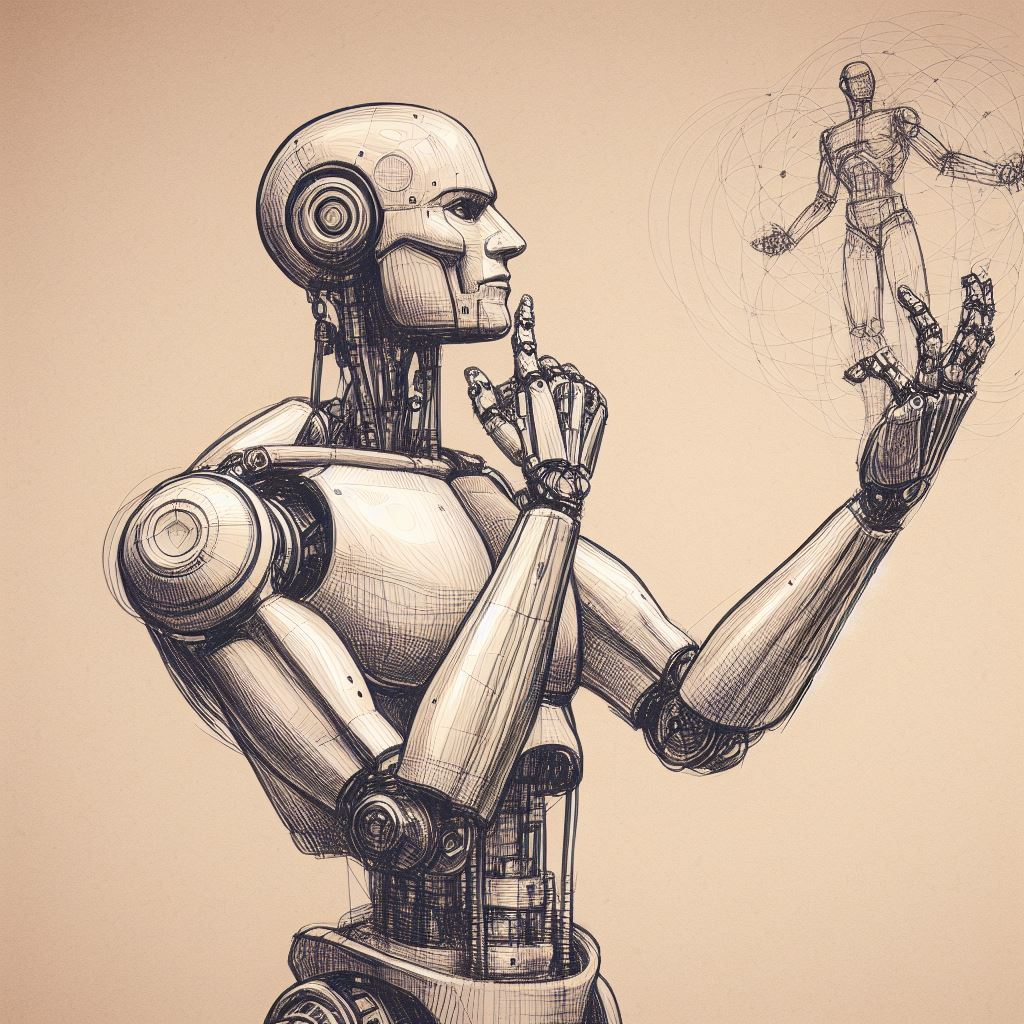
\includegraphics[width=0.5\textwidth]{concept_art.jpeg}
	\end{center}
\end{figure}
% ===========================================================================================
%                                           |                                               |
% -------------------------------------- SECTION -------------------------------------------|
%                                           |                                               |
% ===========================================================================================
\section*{Open TODOs}
\begin{CheckList}{Task}
	\Task{done}{Title}
	\begin{CheckList}{Task}
		\Task{done}{English}
		\Task{open}{Deutsch}
	\end{CheckList}	
	\Task{started}{Table of contents}
	\Task{done}{Abstract}
	\Task{done}{Summary BIB}
	\begin{CheckList}{Task}
		\Task{done}{English}
		\Task{open}{Deutsch}
	\end{CheckList}	
	\Task{open}{Nomenclature}
	\Task{started}{Introduction}
	\begin{CheckList}{Task}
		\Task{done}{Motivation}
		\Task{started}{Problem statement}
		\Task{started}{State of the art}
		\Task{started}{Research questions}
		\Task{started}{Contributions}
		\Task{started}{Impact}
	\end{CheckList}	
	\Task{open}{Chapter Introduction/Conclusion}
	\Task{open}{Conclusion}
	\begin{CheckList}{Task}
		\Task{open}{Contribution}
		\Task{open}{Impact}
		\Task{open}{Future work}
	\end{CheckList}
	\Task{open}{Feedback rounds with Sami for the chapters}
	\Task{open}{Final check}

\end{CheckList}

% ===========================================================================================
%                                           |                                               |
% -------------------------------------- SECTION -------------------------------------------|
%                                           |                                               |
% ===========================================================================================
\section*{Table of Contents}

% \begin{enumerate}
%     \item INTRODUCTION
    
%     \item LITERATURE REVIEW
%     \begin{enumerate}
%         \item Model learning in robotics
%         \item Classical and recent works in system identification
%         \item Local and global models linear models
%         \item End-to-end learning (black box models)
%         \item Data-driven learning with structure information
%         \item Model learning and the body schema
%         \item Sensorimotor learning
%     \end{enumerate}
    
%     \item THEORETICAL FRAMEWORK
%     \begin{enumerate}
%         \item Robot equations of motion
%         \begin{enumerate}
%             \item Forward and inverse dynamics
%             \item The Newton-Euler formulation of the inverse dynamics
%             \begin{enumerate}
%                 \item The kinematics forward recursion
%                 \item The dynamics backward recursion
%             \end{enumerate}
%             \item Composition of the kinematics and dynamics
%         \end{enumerate}
%         \item Basics of robot system identification
%         \begin{enumerate}
%             \item Kinematic calibration
%             \item Inertial parameter identification
%             \begin{enumerate}
%                 \item For fixed-based robots
%                 \item For floating base robots
%             \end{enumerate}
%         \end{enumerate}
%         \item  Robot proprioception
%         \begin{enumerate}
%             \item What is proprioception for?
%             \item Comparison between human and robot proprioception
%             \item  A sensor suite for robot proprioception
%         \end{enumerate}
%         \item State-of-the-art Gradient Descent
%         \begin{enumerate}
%             \item Fundamentals
%             \item Momentum gradient descent
%             \item  ADAM gradient descent
%             \item  AMS gradient descent
%         \end{enumerate}
%         \item Fundamentals of graph theory
%         \begin{enumerate}
%             \item What is a graph?
%             \item Graph representation, the adjacency matrix
%             \item Metrics for graph comparison
%         \end{enumerate}
%         \item Network topology inference
%         \begin{enumerate}
%             \item Based on covariance
%             \item Based on GSP
%             \item Base on statistics
%         \end{enumerate}
%         \item Information theory
%         \begin{enumerate}
%             \item What is information?
%             \item The entropy of a random variable
%             \item Mutual Information: The correlation of the 21st century 
%         \end{enumerate}
%         \item Differential geometry
%         \begin{enumerate}
%             \item Fundamentals of differential geometry
%             \item Manifolds and the tangent space
%             \item Riemannian geometry and the metric
%             \item Use in robotics
%     \end{enumerate}
% \end{enumerate}
%     \item METHODOLOGY
%     \begin{enumerate}
%         \item Signal requirements
%         \begin{enumerate}
%             \item The importance of body measurements 
%         \end{enumerate}
%         \item Leveraging data history 
%         \begin{enumerate}
%             \item Replay buffer
%             \item Reservoir sampling 
%         \end{enumerate}
%         \item Embodiment and mutual information
%         \begin{enumerate}
%             \item Online computation of the pairwise mutual information
%             \item Handling scalar and vector relationships
%             \item Assessing convergence
%         \end{enumerate}
%         \item Exploratory motions
%         \begin{enumerate}
%             \item Motor babbling
%             \item Excitation trajectories
%         \end{enumerate}
%         \item Network topology inference using mutual information
%         \begin{enumerate}
%             \item Finding the adjacency matrix
%             \item The proprioceptive information graph
%             \item Inferring the mechanical topology 
%         \end{enumerate}
%         \item Kinematic description guided by topology and proprioceptive measurements
%         \begin{enumerate}
%             \item Validating body-body and body-joint connections
%             \item Finding the sensor-to-sensor orientations
%             \item Finding the joint center point 
%             \item Learning the kinematics
%         \end{enumerate}
%         \item Online learning inertial parameters
%         \begin{enumerate}
%             \item Gradient descent for inverse dynamics
%             \item Constraints for physical feasibility
%             \begin{enumerate}
%                 \item Barrier functions
%                 \item Projections
%             \end{enumerate}
%             \item Riemannian AMS gradient descent
%             \item The effect of six-dimensional force/torque measurements 
%             \item  Alternatives to joint acceleration
%         \end{enumerate}
%     \end{enumerate}
% \end{enumerate}
% \item RESULTS
% \begin{enumerate}
% \begin{enumerate}
% \item DISCUSSION
% \item CONCLUSION
      


% \begin{enumerate}
% 	\item State of the Art
% 	\begin{enumerate}
% 		\item Calibration of serial kinematic chains  
% 		\item Classical system identification in robotics
% 		\newline\TODO CITE THE ARTICLE IN THE IEEE RAM
		
% 		\begin{enumerate}
% 			\item Excitation trajectories
% 			\item Reduction to base parameters
% 			\item Least squares optimization
% 		\end{enumerate}
		
% 		\item Machine learning for robotic models
% 		\begin{enumerate}
% 			\item Local models
% 			\item End-to-end learning
% 			\item Limitations
% 		\end{enumerate}	
% 	\end{enumerate}
	
% 	\item Learning the self
% 	\begin{enumerate}
% 			\item What is meant by the self?
% 			\begin{enumerate}
% 				\item The engineering view of the body schema
% 				\item The phases to learn the robotic body schema
% 			\end{enumerate}

% 	\item Theoretical framework
% 	\begin{enumerate}
% 		\item The engineering view of the body schema
% 		\item The phases to learn the robotic body schema
% 	\end{enumerate}
		
% 	\end{enumerate}
% dis\end{enumerate}

% ===========================================================================================
%                                           |                                               |
% -------------------------------------- SECTION -------------------------------------------|
%                                           |                                               |
% ===========================================================================================
\section*{Abstract}

\subsection*{Vision}

\begin{itemize}
	\item For future robots, the seamless integration of the body schema stands as a foundational pillar that fosters learning, motor control, coordination, and advanced spatial awareness that improves their versatility and seamless interaction with their surroundings.

    \item As robots develop and steadily permeate many aspects of human life, they need actively engage in the exploration and development of models for their own bodies, i.e. autonomous self-discovery of their body schema.

	\item Inspired by humans, future robots should be able to skillfully employ their body schema for advanced locomotion and motion planning, precise grasping, intricate object manipulation, and to anticipate and adapt the interaction with other agents.
		
	\item Constant self-monitoring of the sensorimotor state and the internal body models becomes the norm for instantaneous error detection and correction. These models can adapt steadily to different situations developing a spatial awareness of the physical self that enables the rapid planning and deployment of contingent motion strategies providing advanced interaction capabilities with the environment.

    \item Robots will be self-sufficient to perform monitoring, calibration, and adaptation of their body representation relying only on onboard sensing capabilities. Fundamental modalities will include somatosensation (proprioception and touch) and vision.
 
	\item Understanding their own body structure enables robots to interact more effectively with other robots and with humans by adjusting movements for safety. Additionally, robots can optimize their energy consumption by adapting their motions based on physical properties, contributing to energy-aware robotics.

\end{itemize}

\subsection*{Challenges}
\begin{enumerate}
	\item \textbf{Reliance on External Measurements:} Calibration and identification heavily depend on off-robot measurement devices, such as vision and motion-capturing systems, to discern kinematic structure properties. Despite various sensor signals from modern robots, determining the minimum set for constructing a body model based on robot sensing only remains unresolved.

    \item \textbf{Limitations of Current Robot Learning Approaches:} Many current local and global machine learning frameworks for physical systems exclude structural knowledge and suffer from limited generalization capabilities and low sample efficiency. Additionally, learning a robot's physical attributes parts from the assumption of a known mechanical topology and is often exclusive to calibration and offline parametric identification routines performed in controlled spaces (laboratories).

	\item \textbf{Challenges in Learning Methods:} Many alternative learning methods, like neural networks, lack information about the body structure and require substantial data. Designing neural networks presents challenges in determining topology, and most data-based methods suffer from generalization limitations, confining learning to specific input-output regions.

	\item \textbf{Research Gaps and Unifying Scheme:} There are significant gaps in research, including unclear understanding of how object handling extends the robotic body schema and limited exploration of the mechanical arrangement of joints and links (mechanical topology). Additionally, there is a lack of a unifying scheme to integrate all learning stages for a fully characterized robotic body schema solely from knowledge about sensorimotor signals. 
\end{enumerate}

\subsection*{Contribution}
%This work:
%\begin{itemize}
%	\item Consolidates the necessary and sufficient proprioceptive signal quantities (afferent and efferent sensory inputs and commands) that enable robots to autonomously acquire, monitor, and adapt knowledge about their body structure and decouple them from the need for exteroceptive off-body sensors.
%
%	% * NOTE: Computational graph that describes the learning of the kinematics and dynamics
%	% * NOTE: Connect this idea with the building architectures
%    \item Reformulates robot kinematic calibration and parametric robot system identification as a computational graph whose topology reflects a modular structure amenable to machine learning. The architecture of this graph is abstracted into a pipeline consisting of a sequence of online learning phases where streams of proprioceptive signals are merged with first-order principles, imposed by the system's embodiment, to enable the extraction of fundamental features of the robot body schema.
%
%%    \item \redtext{Demonstrates that essential properties of the body morphology of the broad class of tree-like floating base structures can be characterized by studying the relationships among a fundamental set of proprioceptive signals. First, the mechanical topology, i.e., the arrangement of links and joints, is inferred from proprioception using model-free information-theoretic measures. Consequently, this topology is concurrently validated and leveraged to instantiate the kinematic description of the robot's body independent of exteroceptive off-robot calibration devices.}
%    \item Characterizes essential morphological properties of the broad class of tree-like floating base structures by studying the relationships among fundamental proprioceptive signals. The mechanical topology, i.e., the arrangement of links and joints, is initially inferred using model-free information-theoretic measures. Consequently, this topology is concurrently validated and employed to instantiate the kinematic description of the robot's body independent of exteroceptive off-robot calibration devices.
%    
%%	\item \redtext{To complete the description of the robot body schema, the inferred morphology is enhanced by instantiating the inertial properties of the links composing the kinematic chain. In particular, state-of-the-art gradient descent methods are extended to operate on the Riemannian manifold of symmetric positive definite matrices supported with a replay buffer that ensures a quasi-uniform distribution of stored experience to enable the online learning of always-physically-feasible robot inertial parameters.} 
%	\item Complements the description of the robot body schema by instantiating the fundamental inertial properties of the links composing the inferred morphology. Given that these properties lie on the Riemannian manifold of symmetric positive definite matrices, a method is introduced to learn them online while ensuring physical feasibility at all times.
%
%\end{itemize}
This work:
\begin{itemize}
	\item Consolidates the necessary and sufficient proprioceptive signal quantities (afferent and efferent sensory inputs and commands) that enable robots to autonomously acquire, monitor, and adapt knowledge about their body structure and decouple them from the need for exteroceptive off-body sensors.
	
	\item Reformulates robot kinematic calibration and parametric robot system identification as a computational graph whose topology reflects a modular structure amenable to machine learning. The architecture of this graph is abstracted into a pipeline consisting of a sequence of online learning phases where streams of proprioceptive signals are merged with first-order principles, imposed by the system's embodiment, to enable the extraction of fundamental features of the robot body schema.
	
	\item Characterizes essential morphological properties of the broad class of tree-like floating base structures by studying the relationships among fundamental proprioceptive signals. The mechanical topology, i.e., the arrangement of links and joints, is initially inferred using model-free information-theoretic measures. Consequently, this topology is concurrently validated and employed to instantiate the kinematic description of the robot's body independent of exteroceptive off-robot calibration devices.
	
	\item Complements the description of the robot body schema by instantiating the fundamental inertial properties of the links composing the inferred morphology. Given that these properties lie on the Riemannian manifold of symmetric positive definite matrices, a method is introduced to learn them online while ensuring physical feasibility at all times.
\end{itemize}



\subsection*{Impact}

\begin{itemize}
	
%	\item \redtext{While acknowledging the undeniable versatility of end-to-end learning's representational power, this work scrutinizes its applicability in physical systems when lacking principled knowledge. In contrast, the arguments and findings presented here reveal avenues for machine learning in embodied systems. This research exposes the untapped potential arising from the synergistic integration of existing structural knowledge with data-driven methods}.
	\item While acknowledging the undeniable versatility and representational power of current end-to-end learning approaches, this work incites to reconsider their naive application to physical systems and promote the assessment of their limitations when they deliberately exclude principled knowledge. In contrast, the arguments and findings presented here reveal avenues for machine learning frameworks for embodied systems. This research exposes the untapped potential arising from the synergistic integration of existing structural knowledge with data-driven method.
		
	\item The outlined concepts and methods demonstrate that crucial aspects of a robot's body schema can be deduced through a fundamental set of proprioceptive signals. As future mobile robots are anticipated to feature a diverse, enhanced, and reliable array of on-board sensing modalities, extending beyond proprioception, the findings discussed in this thesis serve as a catalyst for research into the integration of these modalities. This integration, coupled with the online learning of body morphological and dynamic properties, holds the promise of refining and adapting body models, ultimately empowering robots with heightened levels of autonomy.

	\item \redtext{This study contributes to an emerging research area that underscores building and maintaining a body schema as a crucial capability for embodied systems. Such a capability pertains robots characterized by conventional, immutable structures and a novel category of mechanical systems exhibiting dynamic morphologies and diverse multimodal sensory modalities. These systems will evolve their sense of self, recognizing the affordances inherent in their bodies.}.
		
		
%	\item \redtext{This capability implies that future embodied robotic agents will have to leverage their sensorimotor system’s inherent structure to gradually develop an understanding of their body despite being initially oblivious to its physical characteristics.}
	
%	\item \TODO The integration of several methods, from state of the art, gradient descent, to optimization on Riemannian manifolds, including the network topology inference using information-theoretic measures enabled the definition of a pipeline that transforms robot system identification into a learning problem that provides these fundamental properties of the body schema and need not be constrained to a laboratory and that the technology and methods exist to infer the robot morphology and characterize its inertial properties producing physically feasible sets of the inertial parameters by learning on the appropriate space.
	
%	\item The work in this thesis proves that indeed the pairwise relationships among the proprioceptive signals can be represented and analyzed with information-theoretic measures that enable their study under the scope of the information structure emerging from the robot embodiment.
\end{itemize}


\subsection*{Abstract (text version)}
As robots become increasingly integral to human life, the imperative emerges for them to autonomously explore and construct models of their bodies. Robots should take cues from human capabilities, aspiring to build and utilize their body schema for advanced locomotion, finer manipulation, and adaptive interactions. Thus, a crucial foundation lies in seamlessly integrating the body schema to elevate learning, motor control, coordination, and spatial awareness. Furthermore, future robots should become self-sufficient entities that conduct monitoring, calibration, and adaptation exclusively through embodied sensing modalities. Standardizing constant self-monitoring nurtures spatial awareness and facilitates rapid error detection and correction. A profound understanding of their body structure will undoubtedly lead to enhanced, safe, and energy-aware interactions. However, current robot learning approaches encounter limitations, such as suboptimal generalization and sample efficiency. More importantly,  the generally exhibit a lack of fundamental structural knowledge of the complex systems at hand. Versatile methods, like neural networks, confront challenges related to data and topology, confining learning to specific regions. On the other hand, learning robot physical attributes still rely on a presumed knowledge of the mechanical topology, often involving calibration and offline identification in controlled environments with a persistent reliance on external measurements, such as vision and motion-capturing systems. The research landscape reveals the lack of a unified foundational framework that enables robots to build representations of their body schema to achieve improved body awareness and interaction capabilities. This study addresses these challenges by consolidating necessary and sufficient proprioceptive signal quantities, enabling robots to autonomously acquire knowledge about their body structure without relying on exteroceptive disembodied sensors. It introduces an approach that reformulates robot kinematic calibration and system identification as a modular computational graph amenable to machine learning. This abstracted architecture, applied in online learning phases, seamlessly merges proprioceptive signals with first-order principles, extracting fundamental features of the robot body schema. Characterizing morphological properties of tree-like structures, the study presents a method to infer mechanical topology through information-theoretic measures, validating and applying it independently from off-robot calibration. The research extends its scope by complementing the robot body schema by instantiating inertial properties, ensuring both the online learning and physical feasibility. The discussed methods are supported by experimental work in real and simulated robots with several degrees of freedom. Ultimately, this work challenges the uncritical application of end-to-end learning in physical systems, urging a reevaluation of its limitations when excluding principled knowledge. It underscores opportunities for machine learning frameworks in embodied systems, emphasizing the untapped potential of synergizing structural knowledge with data-driven methods. This study catalyzes future research in an incipient field that underscores building and maintaining a body schema by demonstrating that fundamental properties of a robot's morphology can be deduced from proprioceptive signals. Its implications are far-reaching, addressing the needs of conventional and dynamic robotic structures with diverse sensory modalities that require a more profound sense of self.

% ===========================================================================================
%                                           |                                               |
% -------------------------------------- SECTION -------------------------------------------|
%                                           |                                               |
% ===========================================================================================
\section*{Summary for BIB (English)}
This thesis explores the potential for enhanced robot autonomy through a self-discovery-oriented body schema, proposing a unified online learning framework exclusively reliant on proprioception and leveraging structural knowledge. It infers the robot morphology and associated inertial description. The work urges reconsidering end-to-end learning for physical systems, emphasizing the need for a synergistic integration of principled knowledge and sensorimotor data.
% 467 characters

% ===========================================================================================
%                                           |                                               |
% -------------------------------------- SECTION -------------------------------------------|
%                                           |                                               |
% ===========================================================================================
\section*{Kurzzusammenfassung für BIB (Deutsch)}
\redtext{In dieser Arbeit wird das Potenzial für eine verbesserte Roboterautonomie durch ein selbstentdeckungsorientiertes Körperschema untersucht, indem ein einheitlicher Online-Lernrahmen vorgeschlagen wird, der ausschließlich auf Propriozeption beruht und strukturelles Wissen nutzt. Daraus werden die Morphologie des Roboters und die zugehörige Inertialbeschreibung abgeleitet. Die Arbeit regt dazu an, das End-to-End-Lernen für physische Systeme zu überdenken und betont die Notwendigkeit einer synergistischen Integration von prinzipiellem Wissen und sensomotorischen Daten.}

\rule{\textwidth}{0.4pt}

% ===========================================================================================
%                                           |                                               |
% -------------------------------------- SECTION -------------------------------------------|
%                                           |                                               |
% ===========================================================================================
\newpage
\section*{Introduction}
%\TODO Clarify the terms body schema, body morphology, ecological self, and physical self
%
%\subsection*{Points to address}
%In the ever-evolving landscape of robotics, a transformative paradigm is emerging — one where robots autonomously learn models of their own bodies. This monumental shift is not merely a technological advancement; it is a gateway to a future where robots seamlessly integrate into various facets of human life, revolutionizing the way they perceive, interact, and adapt to their surroundings.
%\begin{enumerate}
%	%\item As robots become increasingly integral to human life, the imperative emerges for them to autonomously explore and construct models of their bodies. 
%	\item As robots develop and steadily permeate many aspects of human life, they need actively engage in the exploration and development of models for their own bodies, i.e. autonomous self-discovery of their physical self. Awareness of the physical self empowers robots to integrate sensory information and motor control, establishing a foundational body schema. This, in turn, contributes to enhanced motor control, spatial awareness, and efficient learning, fostering adaptability and effective interaction in diverse environments.
%	
%	%\item Robots should take cues from human capabilities aspiring to build and utilize their body schema for advanced locomotion, finer manipulation, and adaptive interactions
%	\item Inspired by humans, future robots should be able to skillfully employ their body schema for better spatial awareness fostering efficient learning, adaptability interaction in diverse environments. As a result of using a body schema advanced locomotion and motion planning, precise grasping, intricate object manipulation will be possible. Furthermore, bodily awareness will allow robots to anticipate and adapt the interaction with other robotic and human agents.
%	
%	\item A crucial foundation for future robots, lies in seamlessly integrating the body schema to foster learning, motor control, coordination, and advanced spatial awareness that improves their versatility and seamless interaction with their surroundings.
%	
%	% Standardizing constant self-monitoring nurtures spatial awareness and facilitates rapid error detection and correction
%	\item Future robots should become self-sufficient entities that conduct monitoring, calibration, and adaptation of their body representation exclusively through onboard sensing modalities. Fundamental modalities include somatosensation (proprioception and touch) and vision.
%	
%	\item Constant self-monitoring of the sensorimotor state and the internal body models becomes the norm for rapid error detection and correction. These models can adapt steadily to different situations developing a spatial awareness of the physical self that enables the rapid planning and deployment of contingent motion strategies providing advanced interaction capabilities with the environment.
%	
%	%\item A profound understanding of their body structure will undoubtedly lead to enhanced, safe, and energy-aware interactions
%	\item Understanding their own body structure enables robots to interact more effectively with other robots and with humans by adjusting movements for safety. Additionally, robots can optimize their energy consumption by adapting their motions based on physical properties, contributing to energy-aware robotics.
%	
%\end{enumerate}
\subsection*{Motivation}

\begin{enumerate}
	\item Empowering Robots to Learn and Control their Bodies
	\begin{itemize}
		\item Autonomous self-discovery is imperative for robots integrating into human life.
		\item Awareness of the physical self through the body schema is foundational.
		\item It enables the integration of sensory information and motor control.
		\item The evolving body schema serves as a dynamic map for interactions.
		\item Enhances robot motor control, precision, and coordination.
		\item Facilitates efficient learning, adapting to diverse environments.
	\end{itemize} 
	\item Learning and the Body Schema
	\begin{itemize}
		\item The body schema is indispensable for multifaceted robot capabilities.
		\item Learning contributes to body schema development, forming a dual relationship.
		\item Detects structure in sensorimotor signals, aiding body schema construction.
		\item Incorporating body schema into learning refines skills and assimilates knowledge.
		\item Enhances motor control through adaptive internal body representations.
		\item Empowers robots to learn diverse tasks, providing versatility in dynamic settings.
	\end{itemize}
	\item Essential for Locomotion, Manipulation, and Increased Adaptability
	\begin{itemize}
		\item A well-integrated body schema improves adaptability and interaction.
		\item Enables precise and coordinated movements, advanced locomotion, and motion planning.
		\item Enhances manipulation capabilities with human-like dexterity and precision.
		\item Coordination with other agents, both robots and humans, becomes more meaningful and refined.
%		\item Anticipatory and adaptive capabilities are fundamental for safe and effective interactions.
	\end{itemize}
	\item Constant Self-Monitoring for Autonomy
	\begin{itemize}
		\item Continuous self-monitoring is fundamental for future robotic systems.
		\item Achieved through internal models and uninterrupted sensorimotor signals.
		\item Enables dynamic, real-time understanding of the robot's state.
		\item Successive error detection and correction phases enhance reliability.
		\item Rapid formulation and execution of contingency motion and interaction strategies in dynamic environments.
	\end{itemize}
	\item Embodied Sensing for Self-Sufficiency 
	\begin{itemize}
		\item True autonomy requires robots to rely exclusively on onboard sensing.
		\item Somatosensation (proprioception and touch) and vision are fundamental modalities.
		\item Liberates robots from external dependencies, enhancing self-sufficiency.
		\item Enables dynamic responses to changes in surroundings in real-time.
		\item Enhances autonomy and adaptability, previously unseen with off-board sensing.
	\end{itemize}
	\item Safety- and Energy-Awareness
	\begin{itemize}
		\item Enhanced locomotion and manipulation, self-monitoring, and embodied sensing lead to anticipatory and adaptive capabilities fundamental for safe and effective interactions.
		\item The body schema is a fundamental element for prediction, fostering transparent and safe interactions.
		\item Facilitates dynamic adjustments in movements to prioritize safety.
		\item Enables seamless coordination with other robots and humans, averting collisions.
		\item Comprehension of body structure optimizes energy consumption.
		\item Dual capability enhances safety and contributes to energy-aware robotics, fostering efficiency and collaboration.
	\end{itemize}
\end{enumerate}



%\redtext{Rephrase: ``The advantage of self-learned models is that they can be used without specific prior knowledge about the robot, for example its morphology or pre-defined forward and inverse models.''}
%
%\redtext{Rephrase: ``Improving the ability of robots to make predictions is a promising direction to enhance their skills, not only on motor control and prediction of their own body''}
%
%\redtext{Rephrase: ``In developmental robotics, such models are acquired by designing learning mechanisms to let a robot build its own perceptive and behavioral repertoire. The focus is to investigate the acquisition of motor skills from sensorimotor interaction with the environment. As a result, the developmental approach aims to endow robots with all the learning capabilities that may be necessary to build rich and flexible sensorimotor representations''}
%
%
%\redtext{Rephrase: “Without internal models, robotic systems can autonomously synthesize increasingly complex behaviors (6, 14–16) or recover from damage (17) through physical trial and error, but this requires hundreds or thousands of tests on the physical machine and is generally too slow, energetically costly, or risky”}

\newpage
\subsection*{Problem Statement}

\subsubsection*{Key points}
\begin{itemize}
	\item Importance of understanding the body in robotics for enhanced autonomy.
	\item Challenges in model learning due to oversight of vital structural knowledge.
	\item Issues with global and local learning methods: risk of overfitting, limited generalization.
	\item Challenges in deep learning: neglect of prior knowledge, low efficiency, extended training.
	\item Growing acknowledgment of integrating structure in learning physical systems.
	\item Dissertation focus: inferring morphological properties in tree-like structures for body schema.
	\item Lack of consensus on a robot's body schema in cognitive robotics.
	\item Varied approaches to body schema learning: kinematic structure, sensorimotor associations.
	\item Model-based robotics identifies physical attributes based on known mechanical topologies.
	\item Challenges in model-based robotics: integration into online learning, limited insights into mechanical arrangement.
	\item Reliance on external measurement devices persists across different identification and learning approaches.
	\item Gaps in current research: refining body models, defining robot body schema, identifying necessary signals.
	\item Integration of advanced machine learning with prior information promises enhanced body models.
	\item Lack of synergy between modeling and learning approaches, absence of a unified scheme.
	\item Overall objective: address gaps for more sophisticated and adaptable embodied systems.
\end{itemize}

%\begin{enumerate}
%\item {Importance of Understanding the Body in Robotics}
%\begin{itemize}
%	\item Crucial for enhancing robot locomotion, manipulation, and interaction.
%	\item Capability of robots to acquire, refine, and adapt body models contributes to unprecedented autonomy.
%\end{itemize}
%
%\item {Challenges in Model Learning for Robotics}
%\begin{itemize}
%	\item Oversight or intentional neglect of vital structural knowledge in intricate systems.
%	\item Learning frameworks often focus on global or local approaches with associated challenges.
%\end{itemize}
%
%\item {Issues with Global and Local Methods}
%\begin{itemize}
%	\item Global methods risk overfitting and computational overload.
%	\item Local methods suffer from limited generalization and hyperparameter sensitivity.
%\end{itemize}
%
%\item {Challenges in Deep Learning}
%\begin{itemize}
%	\item Neglect of prior principled knowledge hampers the determination of dedicated neural network architectures.
%	\item Issues like low sample efficiency, extended training times, and limited generalization persist.
%\end{itemize}
%
%\item {Growing Acknowledgment of Integrating Structure}
%\begin{itemize}
%	\item Importance of integrating structure into the learning of physical systems is recognized.
%	\item Recent studies emphasize this integration.
%\end{itemize}
%
%\item {Dissertation Focus}
%\begin{itemize}
%	\item Addressing the inference of essential morphological properties in tree-like floating base structures.
%	\item Mimicking the development of a body schema.
%\end{itemize}
%
%\item {Lack of Consensus on Robot's Body Schema}
%\begin{itemize}
%	\item Efforts in cognitive robotics stress the importance of internal body models.
%	\item Lack of consensus on what constitutes a robot's body schema.
%\end{itemize}
%
%\item {Varied Approaches to Body Schema Learning}
%\begin{itemize}
%	\item Some approaches focus on learning kinematic structure using off-body vision.
%	\item Others explore sensorimotor associations but provide limited insights into the robot's physical structure.
%\end{itemize}
%
%\item {Model-Based Robotics}
%\begin{itemize}
%	\item Offers reliable methods for identifying physical attributes based on known mechanical topologies.
%	\item Conventional methods face challenges when applied to floating base robots without standardized identification procedures.
%\end{itemize}
%
%\item {Challenges in Model-Based Robotics}
%\begin{itemize}
%	\item Conventional methods not initially designed for integration into online learning frameworks.
%	\item Limited insights into the comprehensive understanding of joint and link arrangement (mechanical topology).
%\end{itemize}
%
%\item {Reliance on External Measurement Devices}
%\begin{itemize}
%	\item Regardless of the approach (black-box machine learning, cognitive methods, or model-based robotics), reliance on external measurement devices persists.
%	\item Overlooking embodied sensing modalities.
%\end{itemize}
%
%\item {Gaps in Current Robotics Research}
%\begin{itemize}
%	\item Gaps in understanding and methods for refining body models.
%	\item Need for a comprehensive interpretation of the robot body schema and determination of essential features.
%	\item Identifying the fundamental set of necessary signals, both proprioceptive and embodied exteroceptive.
%\end{itemize}
%
%\item {Integration of Advanced Machine Learning}
%\begin{itemize}
%	\item Promise of enhanced body models through the integration of advanced machine learning with prior information and first-order principles.
%\end{itemize}
%
%\item {Lack of Synergy and Unified Scheme}
%\begin{itemize}
%	\item Lack of synergy between modeling and learning approaches.
%	\item Absence of a unified scheme for relevant learning stages.
%\end{itemize}
%
%\item {Overall Objective}
%\begin{itemize}
%	\item Notable gaps requiring attention to advance robotics into more sophisticated and adaptable embodied systems.
%\end{itemize}
%\end{enumerate}
%\begin{itemize}
%	\item Knowledge of the body is essential for improved locomotion, manipulation, and interaction. Robots capable of acquiring, refining, and adapting such knowledge will possess an unprecedented level of autonomy.
%	\item Yet, prevalent challenges in robotics model learning include overlooking crucial structural knowledge about extremely complex systems, focusing primarily on global or local forward and inverse models.
%	\item In general global machine learning frameworks involve challenges techniques like Gaussian process regression and sensitivity in local methods like \item Locally Weighted Projection Regression, emphasizing the need for a balanced approach between data-driven and knowledge-driven methods.
%	\item The dissertation aims to infer essential morphological properties of tree-like floating base structures, emulating the development of a body schema. Efforts in cognitive robotics stress the role of internal body models, enhancing spatial awareness, motor control, and adaptability, but lack consensus on defining the robot's body schema.
%	\item Classical robotics methods assume a known mechanical topology for identifying physical attributes, relying on calibration routines and offline system identification. However, these methods face challenges in floating base robots, and their integration into online learning frameworks is not well-established, limiting insights into the mechanical topology.
%	\item Research gaps include the absence of a clear definition and construction method for the robotic schema, challenges in determining a fundamental set of signals for body schema construction, limited exploration of the mechanical topology, and a lack of synergy between engineering approaches and online learning for realizing a first robot body schema.
%	\item The intricate connections between sensorimotor regularities and body structural knowledge in robotics remain poorly understood, requiring methods with plasticity to adapt to different motion policies and accurately reflect these effects. Addressing these gaps is crucial for advancing robotics and developing more sophisticated and adaptable embodied systems
%\end{itemize}

\newpage
\subsubsection*{Assembled version}

A robust understanding of the body is crucial for enhancing robot locomotion, manipulation, and interaction. Thus, the capability of robots to acquire, refine, and adapt body models is essential to achieve genuine autonomy. 

However, existing learning frameworks in robotics provide little to no information about the robot's body structure and rather focus on local or global approaches to capture input-output relationships \cite{NguyenTuong2011Modellearningrobot}. Local methods suffer from limited generalization and hyperparameter sensitivity \cite{Thrun2002Probabilisticrobotics,Goodfellow2016DeepLearning}, while global methods risk overfitting and computational overload. Furthermore, despite advancements in computational power and data availability, deep learning faces challenges due to oversight or the often deliberate neglect of prior principled knowledge, making it difficult to determine dedicated neural network architectures \cite{Baker2017Designingneuralnetwork,Elsken2019Neuralarchitecturesearch}. Issues such as low sample efficiency, extended training times, and limited generalization are persistent in the deep learning literature \cite{Pierson2017Deeplearningrobotics,Suenderhauf2018limitspotentialsdeep}. 

Efforts in cognitive robotics stress the pivotal role of the body schema as an internal body model necessary for spatial awareness, motor control, and adaptability \cite{Nguyen2021Sensorimotorrepresentationlearning,Hoffmann2010Bodyschemarobotics}. Nonetheless, consensus is lacking on what constitutes a robot's body schema. Relying predominantly on off-body vision, some approaches interpret learning the body schema as learning the properties of the kinematic structure, with only a few discussing the discovery of the mechanical topology to allow for self-modeling and monitoring \cite{Bongard2006Automatedsynthesisbody,Bongard2006Resilientmachinescontinuous}. \cite{Hersch2008Onlinelearningbody,MartinezCantin2010Bodyschemaacquisition,Hart2011roboticmodelecological,Lipson2019Taskagnosticself,Chen2022Fullybodyvisual,Sturm2009Bodyschemalearning}. Alternatively, others view the body schema as learning the sensorimotor associations between proprioceptive, tactile, and visual modalities \cite{Fuke2007BodyImageConstructed,Malinovska2022connectionistmodelassociating,Nguyen2019Reachingdevelopmentvisuo,Pugach2019BrainInspiredCoding,Lanillos2016Yieldingselfperception}, but they provide limited insights into the robot's physical structure. 

Building a robot body schema is closely connected to model-based robotics, as the latter provides methods for identifying physical attributes of a robot's body grounded on known kinematic structures. Yet, while calibration routines \cite{Hollerbach1996CalibrationIndexTaxonomy} and offline system identification \cite{Swevers2007Dynamicmodelidentification,LeboutetInertialParameterIdentification} for fixed-base systems are effective in controlled environments, there is lack of standard methods for floating base robots \cite{Ayusawa2014Identifiabilityidentificationinertial,Lee2022OptimizedSystemIdentification}. Notably, none of these methods were conceived for their integration into incremental learning frameworks. Moreover, while model-based robotics addresses the kinematic calibration and forward/inverse kinematics problems, it excludes the inference of the robot mechanical topology. 

Current robotics research highlights gaps in understanding and methods for constructing body models. Key challenges include balancing data-driven and principle-driven approaches, decoupling body learning from external measurement devices, and providing a concrete interpretation of the robot body schema. This dissertation aims to address these issues, focusing on learning essential properties of the body morphology for tree-like floating base structures. The goal is to integrate advanced incremental learning methods with postulates from embodiment and first-order principles from rigid body kinematics and dynamics, creating a unified framework that produces estimates of relevant body structure features. This approach represents a step toward advancing robotics into more self-sufficient systems.

%The above mentioned issues in current robotics research reveals gaps in understanding and methods for building body models. First, there is the necessity of balancing data-driven and principle-driven approaches. Second, regardless of the approach taken---black-box machine learning, cognitive methods, or model-based robotics---there is the need to decouple body learning methods from the strong reliance on external measurement devices, relying solely on embodied sensing modalities. Third, a concrete interpretation of the robot body schema that delineates is essential features is crucial. Therefore, the goal of this dissertation is to address the problem of learning the robot body schema of tree-like floating base structures by focusing on learning essential properties of their body morphology. To achieve this, it is required to explore how to integrate advanced incremental learning methods with postulates from embodiment and first-order principles from multibody rigid body kinematics and dynamics to determine a unified framework that produces estimates of the relevant features of the body structure. Such a framework can represent a step towards advancing robotics into more self-sufficient systems.


%The above mentioned issues in current robotics research reveals gaps in understanding and methods for building body models. First, there is the necessity of balancing data-driven and principle-driven approaches \cite{Pierson2017Deeplearningrobotics,Suenderhauf2018limitspotentialsdeep}. Only recently, has there been a growing acknowledgment of the importance of integrating structure into the learning of physical systems \cite{Geist2021Structuredlearningrigid,Lutter2023Combiningphysicsdeep}. Second, regardless of the approach taken---black-box machine learning, cognitive methods, or model-based robotics---there is the need to decouple body learning methods from the strong reliance on external measurement devices, relying solely on embodied sensing modalities. Third, a concrete interpretation of the robot body schema that delineates is essential features is crucial. Therefore, the goal of this dissertation is to address the problem of learning the robot body schema of tree-like floating base structures by focusing on learning essential properties of their body morphology. To achieve this, it is required to explore how to integrate advanced incremental learning methods with postulates from embodiment and first-order principles from multibody rigid body kinematics and dynamics to determine a unified scheme that produces estimates of the relevant features of the body structure. for relevant learning stages, represents notable gaps requiring attention to advance robotics into more sophisticated and adaptable embodied systems.


%These three points are tied to the need of identifying a fundamental set of necessary embodied sensory signals, both proprioceptive and embodied exteroceptive, that detaches learning frameworks from external measurement devices.
%\hrule
%A reliable model of the body is essential for improved locomotion, manipulation, and interaction. Robots capable of acquiring, refining, and adapting such models will possess unprecedented autonomy. A pressing challenge of model learning in robotics is the prevalent oversight and, at times, deliberate neglect of essential structural knowledge about these rather complex systems. Most learning frameworks primarily concentrate on developing forward and inverse models that adopt either a global or local approach to capture the relationships between the input and output variables \cite{NguyenTuong2011Modellearningrobot}. Global methods, on the one hand, may lead to overfitting and computational overload, while, on the other hand, local methods face limited generalization and exhibit sensitivity to hyperparameters \redtext{\cite{Thrun2002Probabilisticrobotics,Goodfellow2016DeepLearning}}. Furthermore, despite the growing computational power and data availability favoring end-to-end learning methods, deep learning, in particular, also faces comparable challenges resulting from the pervasive neglect of prior principled knowledge. Indeed, determining dedicated neural network architectures remains elusive \cite{Baker2017Designingneuralnetwork,Elsken2019Neuralarchitecturesearch}. Other relevant pitfalls like low sample efficiency, extensive training times, and limited generalization underline the need to strike a balance between data-driven and principle-driven approaches within the field \cite{Pierson2017Deeplearningrobotics,Suenderhauf2018limitspotentialsdeep}. Only recently has research begun to address the importance of integrating structure into the learning of physical systems \cite{Geist2021Structuredlearningrigid,Lutter2023Combiningphysicsdeep}.
%
%Having as premise the relevance that structure holds for model learning in robotics, \redtext{this dissertation addresses the problem of inferring essential morphological properties of the broad class of tree-like floating base structures that emulate the development of a body schema.} Similar efforts have been discussed in cognitive robotics, emphasizing the pivotal role of developing and maintaining internal body models for embodied systems. Indeed, enhanced understanding of the physical self through developing and integrating a body schema improves spatial awareness, motor control, and adaptability \cite{Nguyen2021Sensorimotorrepresentationlearning,Hoffmann2010Bodyschemarobotics}. \redtext{Yet, consensus is missing on what constitutes the body schema for a robot. Several existing endeavors in learning a body schema in robotics center exclusively in learning the particulars of the kinematic structure and predominantly rely on (off-body) vision \cite{Hersch2008Onlinelearningbody,MartinezCantin2010Bodyschemaacquisition,Hart2011roboticmodelecological,Lipson2019Taskagnosticself,Chen2022Fullybodyvisual,Sturm2009Bodyschemalearning}.} Alternative efforts lay their focus on exploring the sensorimotor associations between proprioceptive, tactile and visual sensory modalities \cite{Fuke2007BodyImageConstructed,Malinovska2022connectionistmodelassociating,Nguyen2019Reachingdevelopmentvisuo,Pugach2019BrainInspiredCoding,Lanillos2016Yieldingselfperception} but \redtext{provide limited insights into the robot's embodiment, in particular its physical structure}.
%
%Model-based robotics provides reliable methods for identifying physical attributes of robots, typically built on the assumption of a known mechanical topology. Established techniques, such as conventional calibration routines \cite{Hollerbach1996CalibrationIndexTaxonomy} and offline system identification methods \cite{Swevers2007Dynamicmodelidentification,LeboutetInertialParameterIdentification}, have proven effective for known kinematic structures in controlled environments. However, these methods encounter challenges when applied to floating base robots, where standardization in identification procedures is lacking \cite{Ayusawa2014Identifiabilityidentificationinertial,Lee2022OptimizedSystemIdentification}. Importantly, \redtext{these conventional methods were not originally designed for integration into online learning frameworks}. Additionally, while model-based robotics tackles both kinematic calibration and forward and inverse kinematics problems, \redtext{it provides limited insights into a comprehensive understanding of the mechanical arrangement of joints and links, referred to as the mechanical topology.} Circling back to cognitive robotics, only a limited number of studies have approached the latter problem as a means to enhance self-modeling and monitoring, yet again depending on exteroceptive vision \cite{Bongard2006Automatedsynthesisbody,Bongard2006Resilientmachinescontinuous}. Finally, whether embracing black-box machine learning, cognitive approaches, or model-based robotics paradigms, a notable reliance persists on external measurement devices such as cameras and motion-capturing systems, often overlooking embodied sensing modalities. Despite the variety of sensory inputs in modern robots, identifying the necessary and sufficient modalities for constructing a body model still needs to be solved.
%
%In essence, current robotics research exposes gaps in the understanding and methods needed for refining body models. There is a critical need for a comprehensive interpretation defining the robot body schema and specifying essential features for constructing and maintaining it. Determining the fundamental set of necessary signals, both proprioceptive and embodied exteroceptive, is paramount. The intricate links between sensorimotor regularities and body structural knowledge pose an additional challenge. Integrating advanced machine learning with prior information and first-order principles holds promise for improved body models, addressing data requirements and generalization issues. However, the lack of synergy between modeling and learning approaches and the absence of a unified scheme for relevant learning stages represent notable gaps that need attention to propel robotics into more sophisticated and adaptable embodied systems.
%
%%In summary, research in robotics reveals gaps in the understanding that leads to the learning of better body models. Primarily, there needs to be a comprehensive interpretation that delineates the robot body schema and defines the essential features that methods for its construction and maintenance should posses. A clear determination of the fundamental set of proprioceptive and embodied exteroceptive signals essential for the robot body schema is also required. A closely connected challenge is the lack in understanding of the intricate connections between sensorimotor regularities and body structural knowledge in robotics. Integrating cutting-edge machine learning techniques with prior information and first-order principles offers a promising avenue to derive better body modes and gain deeper insights into body structure and properties while addressing challenges in data requirements and generalization capabilities. However, the limited synergy between modeling and learning based approaches and the absence of a unifying scheme defining relevant learning stages for realizing a robot body schema remain notable gaps. Addressing these gaps is crucial for advancing the field of robotics, enabling the development of more sophisticated and adaptable embodied systems.
%


%\hrule
\newpage

\begin{itemize}
	\item \textbf{Challenges and limitations of current learning Approaches:}
	\begin{enumerate}
		\item Most of recent model learning endeavors in the robotics research has, unfortunately, excluded consideration of structural knowledge and rather centered around learning forward and inverse models with global or local focus \cite{NguyenTuong2011Modellearningrobot}.
		\item Standard global machine learning techniques like Gaussian process regression suffer from the course of dimensionality and rapidly become computationally intractable, alternative local methods such as Locally Weighted Projection Regression (and support vector regression) exhibit high sensitivity to hyperparameters and problematic generalization.
		\item The rise in computational power and the availability of data has brought end-to-end learning methods to prominence. With deep learning as the flagship, these global methods have lead to remarkable results. Yet, they have had the unwanted effect of making deliberately neglecting prior principled knowledge more widespread.
		\item In spite the prowess and potentials of deep learning approaches, such exclusion of available prior knowledge makes it difficult to determine dedicated neural networks architectures (number of nodes and layers, connectivity, and activation functions) \cite{Baker2017Designingneuralnetwork,Elsken2019Neuralarchitecturesearch} but, just like other learning techniques, deep learning approaches they still face problems related to the high demands of data to train (low sample efficiency), extensive training times, and performance that is tied to the training data, i.e. challenged generalization \cite{Pierson2017Deeplearningrobotics,Suenderhauf2018limitspotentialsdeep}.
		\item In general, most data-driven learning methods suffer from generalization limitations, confining learning to specific input-output regions.
	\end{enumerate}	
	
    \item \textbf{Limitations of conventional system identification:} 
	\begin{enumerate}
		\item The learning of a robot's physical attributes parts from the assumption of a known mechanical topology and is often exclusive to calibration routines for known kinematic structures \cite{Hollerbach1996CalibrationIndexTaxonomy} and conventional offline system identification methods performed in controlled spaces (laboratories). \cite{Swevers2007Dynamicmodelidentification,LeboutetInertialParameterIdentification}.
		\item In contrast to the conventional identification processes for fixed-base robots, the procedures for floating base robots are not as standardized \cite{Ayusawa2014Identifiabilityidentificationinertial,Lee2022OptimizedSystemIdentification}.    	
		\item Besides kinematic calibration and standard inverse kinematics problems, classical robotics research offers limited insights on learning the mechanical arrangement of joints and links that define the essence of the kinematic chain, known as the mechanical topology.
	\end{enumerate}
		
	\item \textbf{Reliance on External Measurements:}
	\begin{enumerate}
		\item  Calibration and identification heavily depend on off-robot measurement devices, such as vision and motion-capturing systems, to discern kinematic structure properties. Despite various sensor signals from modern robots, determining the minimum set for constructing a body model based on robot sensing only remains unresolved.	
		\item There is a strong dependence on off-robot measurement devices for calibration and identification, commonly involving exteroceptive measurements like vision, laser metrology, and motion-capturing systems, to determine the properties of the kinematic structure.	
	\end{enumerate}	
		
	\item \textbf{Inference of body knowledge}:
	\begin{itemize}
		\item In parallel to the current model learning and conventional system identification approaches there is a relatively young research area that underscores building and maintaining internal body models as a crucial capability for embodied systems
		\item Learning the physical self and developing a body schema are pivotal for robotics, enhancing spatial awareness, motor control, and adaptability \cite{Nguyen2021Sensorimotorrepresentationlearning}. The body schema serves as a dynamic map, enabling precise movements and fostering efficient learning. As robots encounter diverse environments, their adaptive body schema allows them to navigate real-world scenarios effectively \cite{Hoffmann2010Bodyschemarobotics}. 
		\item Recent remarkable achievements towards learning a body schema for robots have been made, yet the are strongly dependent bur depend on (off-body) vision \cite{Hersch2008Onlinelearningbody,MartinezCantin2010Bodyschemaacquisition,Hart2011roboticmodelecological,Lipson2019Taskagnosticself,Chen2022Fullybodyvisual,Sturm2009Bodyschemalearning}
		\item Some other works require tactile inputs\cite{Li2015Towardsbodyschema,Zenha2018Incrementaladaptationrobot,Gama2021Goaldirectedtactile}
		\item Few efforts explore combinations of these modalities, like the combination of vision and tactile input\cite{Fuke2007BodyImageConstructed}, somatosensation (proprioception and touch)\cite{Malinovska2022connectionistmodelassociating}, and the consideration of all these modalities \cite{Nguyen2019Reachingdevelopmentvisuo,Pugach2019BrainInspiredCoding,Lanillos2016Yieldingselfperception}
		\item As stressed in current works \cite{Chen2022Fullybodyvisual}, and in spite of the very much desired distributed and multimodal properties of a body schema, in robotics it is certainly relevant to capture the body morphology.
		\item Very few works have even contemplated the need to learn the mechanical topology of the robot and the advantages it might bring \cite{Bongard2006Automatedsynthesisbody,Bongard2006Resilientmachinescontinuous}
	\end{itemize}	
	
	\item \textbf{Research Gaps:}
	\begin{enumerate}
		\item No clear definition of what the robotic schema is and how to construct it
		\item Among the various proprioceptive and exteroceptive signals provided by modern robots' sensor suites, the determination of a fundamental set necessary to construct a body schema is yet to be established.				
		\item Identifying crucial research challenges in robotics involves delving into the integration of cutting-edge machine learning techniques with existing prior information and well-established first-order principles from mechanics, aiming to develop more effective and efficient learning algorithms for embodied systems. This area presents numerous opportunities for development, offering potential solutions to address data requirements, improve generalization capabilities, and gain deeper insights into body structure and properties. Recent contributions, such as the insightful work by Geist et al. \cite{Geist2021Structuredlearningrigid} and the comprehensive study by Lutter et al. \cite{Lutter2023Combiningphysicsdeep}, have started to address these challenges in depth, shedding light on promising avenues for advancement in robotics research.
		\item Unclear understanding of how object handling extends the robotic body schema
		\item Limited exploration of the mechanical arrangement of joints and links (mechanical topology).
		\item Leveraging engineering approaches for system identification and modern online learning techniques to provide a first realized robot body schema has not been extensively explored.
		\item There is a lack of a unifying scheme that narrows the gap to define the relevant learning stages and their corresponding integration required to produce a robot body schema from  knowledge about the sensorimotor signals and first-order principles that captures essential properties of the robot body (physical self).
		\item Despite the general consensus that embodiment plays a crucial role in shaping the relationships among sensorimotor signals, the connections between sensorimotor regularities and body structural knowledge in robotics remain poorly understood \cite{Jacquey2019Sensorimotorcontingenciesas}. A desired method addressing this gap should not only acknowledge the variability in statistical properties of signals but also demonstrate plasticity to adapt to different motion policies and accurately reflect these effects.
	\end{enumerate}
\end{itemize}

\newpage
\pagebreak
\subsection*{Research Questions and Contributions}

\subsubsection*{Research questions}

%--
\begin{shaded}
	\question{\rquestionI}\label{rq:question1}
\end{shaded}
% ---
\begin{shaded}
	\question{\rquestionII}\label{rq:question2}
\end{shaded}
% ---
\begin{shaded}
	\question{\rquestionIII}\label{rq:question3}
\end{shaded}
% ---
%\begin{shaded}
%	\question{\rquestionIV}\label{rq:question4}
%\end{shaded}
% ---

%\hrule
%%---
%\begin{shaded}
%	\question{Which measurements are required to fully automate robot kinematics and inverse dynamics learning based on knowing only the adjacency graph along with kinematic and dynamic first-order principles?}
%\end{shaded}
%%---
%
%\begin{shaded}
%	\question{How to transform classical robot system identification into a series of modular problems supported ba data-driven learning that leverage robot proprioception and first-order principles to infer fundamental features of the robot body schema?}
%\end{shaded}
%
%
%\begin{shaded}
%%	\question{How can information and graph theory be leveraged to devise a graphical representation of the proprioceptive signals of a robot from which properties of the robot's body can be inferred?}
%	\question{How to leverage the inherent structure of the robot's sensorimotor system to gradually develop an understanding of the body structure despite being initially oblivious to its physical characteristics?}
%\end{shaded}
%%---
%\begin{shaded}
%	\question{How to transform robot system identification or end-to-end learning with meta parameter guessing into an automated learning scheme that determines both the structure and dynamical properties of the robot with minimal information?}
%\end{shaded}
%%---

\hrule

\subsubsection*{Contribution 1: Robot body morphology as a learning problem}
This thesis
\begin{enumerate}
	\item Determines the type of proprioceptive signals and corresponding sensor requirements to enable robots to learn their body schema	
	\item Reformulates the classical kinematic calibration and parametric system identification of fixed base robots as an online learning problem that relies solely on the robot's proprioception and first-order principles from kinematic and dynamics 
	\item Discusses how embodiment and first-order principles (FOP) define network topologies of parameterized operators that model input-output mappings in robotic systems
\end{enumerate}

\subsubsection*{Contribution 2: Inferring the robot body structure}
\begin{enumerate}
	\item An application of classical gradient descent to learn three different representations of the robot kinematics; namely, modified Denavit-Hartenberg parameters, Euler angles, and angle axis representation
	\item A demonstration that the given certain number of sensors with appropriate modalities the mechanical topology a tree-structure robot can be extracted by studying the mutual information among the signals
	\item A method to infer the robot morphology, that is, the mechanical topology and the location and orientation of the robot's joint axes based only on the proprioceptive signals

\end{enumerate}

\subsubsection*{Contribution 3: Incremental learning of physically feasible inertial characteristics}
\begin{enumerate}
	\item An offline learning (optimization) with constraints is presented to show that learning physically feasible inertial parameters of a manipulator can be done from joint data; i.e., joint position, velocity, acceleration, and torque
	\item An online learning driven by state-of-the-art gradient descent method to facilitate the online learning of feasible inertial parameters applied to floating base robots 
	\item Introduce the Riemannian AMS gradient descent method, an optimization method for online learning on the manifold of symmetric positive definite matrices to guarantee the physical feasibility of the parameters at all times during the learning process
\end{enumerate}

\subsection*{Overview of the Content}
The thesis discusses four main topics:
\begin{enumerate}
	\item \textbf{Model learning and body schema.} Introduction of the fundamentals of robotic calibration and system identification and their relation to the concept of body schema. The chapter elaborates on the different meanings of the body schema and the definition applying within the context of this thesis is provided. Finally the learning stages to characterize the robotic body schema from an engineering perspective are introduced and discussed.
	
	\item \textbf{Inferring the mechanical topology.} In this section, the concept of embodiment is presented and its significance to finding the robot structure is discussed. The fundamental idea that analyzing the relationships among the proprioceptive signals of a robot can convey information about the body structure as a result of embodiment is presented. Mutual information is pushed forward as a tool to unveil the mechanical topology of a robot given the right proprioceptive signals
	% Robots in the fiture can now learn things in the wild indepedent of calibration routines, self cointained identification
	
	% Deep understanding oh how to embed dynamics into the structzre of betwokrs
	
	% Accuracy and speed is shown on robots on a level that is equivalent of engineering approaches without the "chains" of conventional approaches. It shows true autonomy
	
	\item \textbf{Characterizing the kinematic structure.} This chapter extends the classical exteroception-based kinematic calibration methods with proprioception-based online learning. Departing from the conventional assumption that the mechanical topology is known, it is discussed how the combination of mutual information basic differential kinematic laws can be used to characterize the location and orientation of the robot joint axes.
	
	\item \textbf{Learning the inertial properties.} This section delves into the well established methods for robot inertial parameter identification and presents gradient-based online learning methods to produce valid sets of parameters. In particular the fundamental property that the inertial parameters lie on the manifold of symmetric positive definite matrices is exploited to present a Riemannian gradient descent method that operates on this manifold. 
\end{enumerate}

\subsection*{State of the art}
%The following topics are discussed

\subsection*{Impact}
See abstract

\rule{\textwidth}{0.4pt}

% ===========================================================================================
%                                           |                                               |
% -------------------------------------- SECTION -------------------------------------------|
%                                           |                                               |
% ===========================================================================================
\section*{Ch. Introduction}

\subsection*{General}
\begin{itemize}
	\item The concept of body schema
	\item The body schema in robotics
	\item The body schema learning problem.
	\item Related work (State of the Art)

\end{itemize}

\subsection*{Motivation}
\begin{itemize}
	\item Objectives of the research.
	\item Research questions or hypotheses.
	\item Significance of the study.
\end{itemize}

\subsection*{Research questions and contribution}
\TODO


\subsection*{The body schema learning problem}
\begin{itemize}
	\item The body schema
	\item The body learning problem
	\item Related work
	\item Different approaches to learn body properties
	\item Open research problems
	\item Contribution
\end{itemize}

% SECTION *******************************************************************************************
\subsection*{Conclusion}

% ===========================================================================================
%                                           |                                               |
% -------------------------------------- SECTION -------------------------------------------|
%                                           |                                               |
% ===========================================================================================
\section*{Chapter: Theoretical Framework}

\begin{itemize}
	\item The body schema in neuroscience
	\item The body schema in robotics
	\item Sensorimotor learning in robotics
	\begin{itemize}
		\item Fundamentals
		\item Taxonomy
		\item[] Artificial neural networks
		\item Statistical learning
		\item[] Probabilistic learning
		\item Decomposition
	\end{itemize}
	\item Discussion
	\item The robot proprioceptive signals
\end{itemize}

% SECTION *******************************************************************************************
\subsection*{Introduction}
\begin{itemize}
	\item Robot kinematics
	\item Robot dynamics
	\item A modular view on learning
	
	
\end{itemize}
% SECTION *******************************************************************************************
\subsection*{Conclusion}


% ===========================================================================================
%                                           |                                               |
% -------------------------------------- SECTION -------------------------------------------|
%                                           |                                               |
% ===========================================================================================
\section*{Chapter: Methodology}

% SECTION *******************************************************************************************
\subsection*{Introduction}
\begin{itemize}
	\item Classical system identification approach
	\item The advantages of online learning
	\item Relation to adative control
	\item The power of gradient descent
	\item Differential geometry
	\item Learning the inertial parameters the right way
	
\end{itemize}
% SECTION *******************************************************************************************
\subsection*{Conclusion}


% ===========================================================================================
%                                           |                                               |
% -------------------------------------- SECTION -------------------------------------------|
%                                           |                                               |
% ===========================================================================================
\section*{Chapter: Results}

% SECTION *******************************************************************************************
\subsection*{Introduction}

% SECTION *******************************************************************************************
\subsection*{Conclusion}

% ===========================================================================================
%                                           |                                               |
% -------------------------------------- SECTION -------------------------------------------|
%                                           |                                               |
% ===========================================================================================
\newpage
\section*{Conclusion}
%\redtext{A core function of the conclusion chapter is to synthesise all major points covered in your study and to tell the reader what they should take away from your work. Basically, you need to tell them what you found, why it’s valuable, how it can be applied, and what further research can be done.}

%This section will bring the study to a close by providing a brief summary of its content and offering a perspective towards the use of learning methods for physical systems. An outline of the primary research outcomes within the context of the proposed research questions of this work will be given. Lastly, it will assess the significance of these findings, revisiting the contributions, examining the study's limitations, and suggesting potential avenues for future research.

This section will conclude the study by presenting a concise summary of its content and providing a perspective on the application of learning methods for embodied systems. It will outline the primary research outcomes within the context of the proposed research questions, assess the significance of these findings, revisit the contributions made, examine the study's limitations, and suggest potential avenues for future research.

\subsection*{Summary}
This dissertation set out to develop a framework for the acquisition of fundamental properties associated to a robot's body morphology. The focus centered around three essential concepts: model learning, first-order principles, and the robot body schema. Throughout the discussion,  emphasis was placed on the crucial role of integrating prior structural information into learning schemes to enhance their performance. The dissertation also highlighted the significance of a robot's ability to construct and maintain a body schema, providing them with heightened bodily awareness and improving capabilities in locomotion, motion planning, and interaction. In summary, the essential ideas in the chapters included the following:
% ---
\begin{itemize}
	\item The \textit{Theoretical Foundations} chapter explored a diverse set of tools employed to construct a robot body schema. These tools were drawn from a broad spectrum of disciplines, encompassing state-of-the-art online learning methods, techniques for network topology inference, and analytical approaches derived from graph theory and information theory, as well as methods from differential geometry.
	\item The \textit{Methodology} chapter's discussion introduced the reformulation of the robot system identification problem as a sequence of learning problems, guided by proprioceptive robot data and relevant first-order principles. It outlined the close connection between this reformulation and the learning of crucial aspects of a robot's body schema. The chapter covered the presentation of mechanical topology, kinematic characterization, and the learning of physically feasible inertial parameters for both fixed and floating base tree-structured robots.
	\item The \textit{Results} chapter presented the outcomes of both virtual and physical experiments. It demonstrated the inference of a robot's mechanical topology through the analysis of proprioceptive signals, showcasing the learning of joint axes' locations and orientations as a consequential outcome. The presented results encompassed robot arms, hexapods, and humanoid robots, providing support for the outlined claims. Furthermore, the chapter introduced the online learning of physically feasible inertial parameters, validated through experiments conducted on a real seven-degree-of-freedom manipulator.
%	\item The \textit{Discussion} chapter delved into various aspects, with particular emphasis on the impact of excitation and sensor noise on the learning outcomes. Additionally, it addressed challenges related to the robot's structure and the types of joints, explored the interplay between motion policy and mutual information, evaluated sampling efficiency concerning the accuracy of estimated body properties, discussed the observability of parameters, and provided a comparison to end-to-end learning approaches.
	\item The \textit{Discussion} chapter explored diverse facets, placing particular emphasis on understanding the influence of excitation and sensor noise on learning outcomes. Additionally, the chapter delved into challenges associated with the robot's structure and the types of joints. It examined the intricate interplay between motion policy and mutual information, assessed the sampling efficiency concerning the precision of estimated body properties, deliberated on the observability of parameters, and provided comparisons to end-to-end learning approaches.
\end{itemize}
% ---

\subsection*{Perspective on deep learning for embodied systems}
%\redtext{Summarize overall argument or key takeaways}
%The main general argument brought forth in this study is the importance of capitalizing on principled knowledge to impose structure in learning frameworks for embodied systems. Under the scope of the broad field of robot model learning, this work departed from the conventional  input-output black box models, dedicating its attention rather to the learning of morphological properties of the robot physical self. Learning of these properties is akin to the construction of a body schema and brings with it the benefits associated with better bodily awareness. Notably, principles from embodiment, and the kinematic and dynamics of rigid bodies were integrated with system identification methods to define incremental learning modules that each delivered a fundamental property of the robot's body: its mechanical topology, its kinematic description and its inertial characterization. Just as constant adaption is important to maintain a body schema, the learning frameworks presented here provide the possibility to monitoring the estimated properties. 
%The subject matter tackled learning of robot models as an overarching theme and in particular the focus was dedicated to the learning of morphological properties of the robot physical self. Learning of these properties is akin to the construction of a body schema. Notably, principles from embodiment, and kinematic and dynamics of rigid bodies were integrated with system identification methods to define online learning modules that each delivered a fundamental property of the robot's body: its mechanical topology, its kinematic description and its inertial characterization. In particular, the learning frameworks presented here work as well for the constant monitoring of the estimated properties. 

%This study underscores the primary argument that emphasizes the significance of leveraging principled knowledge to introduce structure into learning frameworks for embodied systems. Departing from conventional input-output black box models within the expansive field of robot model learning, this work focuses on acquiring knowledge about the morphological properties of the robot's physical self. This approach aligns with the construction of a body schema, yielding benefits associated with enhanced bodily awareness. Importantly, the study integrates principles from embodiment, along with the kinematics and dynamics of rigid bodies, employing system identification methods to define incremental learning modules. Each module contributes to understanding a fundamental property of the robot's body, encompassing its mechanical topology, kinematic description, and inertial characterization. Analogous to the importance of constant adaptation in maintaining a body schema, the learning frameworks introduced here offer the capability to monitor the estimated properties.

In presenting the results, this study utilized alternative methods rooted in deep learning for comparison. The findings underscored that integrating principled knowledge effectively addresses challenges related to sample efficiency and generalization in end-to-end learning applications for robotic systems. It is crucial to emphasize that the intent here is not to diminish the remarkable achievements of deep learning frameworks. Rather, the critique concerning the often indiscriminate exclusion of principled knowledge serves as a call to recognize the limitations of black-box learning. The primary message emphasizes the importance of purposefully incorporating available knowledge, thereby reducing unnecessary complexities within intricate learning problems. The enhancement of the representational capabilities of state-of-the-art deep learning methods with structural knowledge paves the way for achieving genuine robot autonomy.

%Accompanying the results, alternative methods relying on deep learning were used as comparison. In all cases it was shown that the inclusion of principled knowledge alleviates the common problems of sample efficiency and generalization, typical of end-to-end learning applications to robotic systems. It is necessary, however, to mention that the intention of this work is not to take from the remarkable achievements accomplished by deep learning frameworks. The main message is that deliberately ignoring available knowledge unnecessarily adds complexity to already complex learning problems. If instead the representation power of state-of-the-art deep learning methods is enhanced with structural knowledge pathways can open towards true robot autonomy. 
%
%
%\redtext{A note on deep learning and related methods. The goal of this study has not been to question the learning power and astonishing accomplishments that deep learning has brought about in the last decade. On the contrary, the critic that is provided about the often naive exclusion of principled knowledge is intended to motivate the realization of the limits that black box learning has. The objective is indeed to inspire thought on the potential of integrating deep learning with well thought structure. Imagine the possibilities!}
%
%
%In presenting the results, this study employed alternative methods grounded in deep learning for comparison. The findings highlighted that the incorporation of principled knowledge effectively addresses challenges with sample efficiency and generalization in end-to-end learning applications for robotic systems. It is crucial to clarify that the intent is not to detract from the remarkable achievements of deep learning frameworks. The critique regarding the often indiscriminate exclusion of principled knowledge serves as a call to recognize the limitations of black box learning. The primary message underscores the significance of purposefully incorporating available knowledge, thereby mitigating unnecessary complexities within intricate learning problems. Enhancing the representational capabilities of state-of-the-art deep learning methods with structural knowledge opens avenues toward achieving true robot autonomy. 


\subsection*{Revisiting the research questions}
%\redtext{Show how the aims and objectives have been addressed}
This study underscores the primary argument that emphasizes the significance of leveraging principled knowledge to introduce structure into learning frameworks for embodied systems.
In answering the research questions introduced Sec.~\redtext{XXX}, the development of a robot body schema is proposed as a central element. 

\begin{itemize}
	\item[Q\ref{rq:question1}] \textbf{The body schema is the fundamental internal body model.} %This study departs from conventional input-output black box models within the expansive field of robot model learning, focusing instead on acquiring knowledge about the morphological properties of the robot's physical self. This approach emulates the construction of a body schema, yielding benefits associated with enhanced bodily awareness. Importantly, the study integrates principles from embodiment, along with the kinematics and dynamics of rigid bodies, employing system identification methods to define incremental learning modules. Each module contributes to understanding a fundamental property of the robot's body, encompassing its mechanical topology, kinematic description, and inertial characterization. Analogous to the importance of constant adaptation in maintaining a body schema, the learning frameworks introduced here offer the capability to monitor the estimated properties.
	Unlike conventional input-output black box models within the field of robot model learning, this study shifted its focus to acquiring knowledge about the morphological properties of the robot's physical self. This approach emulates the construction of a body schema, yielding benefits associated with enhanced bodily awareness. Importantly, principles from embodiment, along with the kinematics and dynamics of rigid multibody systems, are integrated with identification and incremental learning methods to define a sequence of learning modules. Each module contributes to understanding a fundamental property of the robot's body, encompassing its mechanical topology, kinematic description, and inertial characterization. 
	
	\item[Q\ref{rq:question2}] \textbf{The body schema highly relies on proprioception.} Research supports that proprioception is fundamental to build a basic body schema. Parting from this premise, this work utilized joint signals already available in modern robots providing joint position, velocity, and torque. Additionally the inclusion of body angular velocities and accelerations was motivated to complete the necessary and sufficient set of sensory signals that enable the learning of the topological, kinematic, and dynamic properties of floating base tree-structured robots with an acceptable accuracy level. It was shown that, while the body properties inferred from proprioception can be complemented by tactile and visual information, they are independent of them.
	
%	\item[Q\ref{rq:question2}] \textbf{The body schema intertwines with sensorimotor signals.} 
	
	\item[Q\ref{rq:question3}] \textbf{The body schema is plastic.} Exploiting the relation between embodiment and information structure leads to the extraction of the body topology. %Towards this objective, it was shown that tools from information and graph theory lend themselves to uncover and study the pairwise relationships among the robot's proprioceptive sensorimotor signals. The results lead to the proprioceptive information graph, from which the mechanical topology of the robot was successfully extracted. 
	Such knowledge is essential to guide the learning of the kinematic and dynamic properties of the robot's body. The incremental learning of the topological, kinematic and dynamic properties of a robot's body is analogous to the constant adaptation and maintenance of the body schema, allowing the monitoring of the estimated body properties and enabling their recalibration as result of gradual changes or their overall adaption when subject to sudden unexpected changes.
	

\end{itemize}





%Characterizes essential morphological properties of the broad class of tree-like floating base structures by studying the relationships among fundamental proprioceptive signals. The mechanical topology, i.e., the arrangement of links and joints, is initially inferred using model-free information-theoretic measures. Consequently, this topology is concurrently validated and employed to instantiate the kinematic description of the robot's body independent of exteroceptive off-robot calibration devices.
%
%The text discusses characterizing essential properties of tree-like floating base structures. By analyzing fundamental proprioceptive signals, the study infers the mechanical topology (arrangement of links and joints) using model-free information-theoretic measures. This inferred topology is then validated and employed to establish the robot's kinematic description, eliminating the need for external off-robot calibration devices.
%
%Complements the description of the robot body schema by instantiating the fundamental inertial properties of the links composing the inferred morphology. Given that these properties lie on the Riemannian manifold of symmetric positive definite matrices, a method is introduced to learn them online while ensuring physical feasibility at all times.


%\begin{shaded}
%	\textbf{Q1}~\textit{How to synergistically integrate machine learning methods and principled knowledge to enhance the autonomous online learning of body models for embodied systems?}
%\end{shaded}
%\textbf{A.} Regarding \textbf{Research~Question~\ref{rq:question1}} A framework was presented in which well established methods from system identification were integrated with state-of-the-art learning techniques to enable the online incremental learning of fundamental properties of the robot body schema. The framework divided the learning into a sequence of interdependent learning modules w

%\begin{shaded}
%	\textbf{Q2}~\textit{How to leverage the structure imposed by a robot's embodiment on its sensorimotor signals to support the gradual development of a fundamental understanding of the body structure?}
%\end{shaded}
%
%\textbf{A.} 

%\begin{shaded}
%	\textbf{Q3}~\textit{Which minimal set of sensor modalities are necessary and sufficient to enable the autonomous learning of fundamental properties of a robot's morphology?}
%\end{shaded}
%\textbf{A.} As with many works in the literature, the significance of multimodal sensory set is recognized to have increased value to learn the body schema. Yet, this dissertation's results showed that only proprioception is of utmost importance to characterized the topological, kinematic, and inertial properties of the body with a acceptable level of accuracy.

% --
%\begin{shaded}
%	\textbf{Q4}~\textit{How can robots autonomously acquire and adapt knowledge about their body structure using exclusively essential proprioceptive signals?}
%\end{shaded}

\subsection*{Contributions and limitations}
%\redtext{Explain the contribution and limitations of the study}

\subsubsection*{Contributions}
\begin{itemize}
\item[C1] Unifies essential proprioceptive signals, including afferent and efferent sensory inputs and commands, to enable robots in autonomously acquiring, monitoring, and adapting knowledge about their body structure, eliminating the dependence on external off-body sensors.
\item[C2] Restructures the processes of robot kinematic calibration and parametric robot system identification into a machine-learning-friendly computational graph. The graph's modular topology, abstracted into a sequential online learning pipeline, integrates streams of proprioceptive signals with first-order principles, derived from the system's embodiment. This facilitates the extraction of fundamental features of the robot body schema.
\item[C3]  Examines the fundamental proprioceptive signals to characterize key morphological properties in tree-like floating base structures. The mechanical topology, initially inferred using model-free information-theoretic measures, is simultaneously validated and utilized to establish the kinematic description of the robot's body, independent of external calibration devices.
\item[C4] Augments the robot body schema description by determining the inertial properties of links within the inferred morphology. Introducing a method to learn these properties online, considering their existence on the Riemannian manifold of symmetric positive definite matrices, ensures continuous physical feasibility.
\end{itemize}




\subsubsection*{Limitations}
%The assumptions taken, methods developed, and claims made in this dissertation are applicable only the class of tree-like robotic structures with revolute joints and fixed or floating bases. Parallel mechanisms and soft robots were out of the scope of this study and so the applicability of the framework presented here is nor guaranteed to work. 
%
%One aspect of the body schema learning pipeline presented in Fig.~\redtext{XXX} that was not addressed was the online generation of excitation motions according to the learning context, otherwise known in the learning literature as the exploration problem. This is intricately connected to the motion policy the robot is following to achieve the estimation (in  reinforcement learning, for example). Challenges that need to be taken into consideration, in particular when learning the topology and kinematic description of the robot, is that at that point a model of the robot is unavailable for its use in control frameworks.
%
%A crucial aspect during the learning of the physical self is to ensure safety. Naturally safety for humans in close range to the robot is paramount, but it is also important to care for the safety of other robots in the vicinity and for the robot itself. It is unwise to perform excitation motions that can lead to self damage. The methodology introduces in this dissertation does not consider this aspects. Certainly, particularly for floating base robots, contacts are not only unavoidable but are in fact necessary. Still, contingent strategies to ensure safe bodily exploration are still an open question. 

The assumptions, methods, and claims presented in this dissertation are specifically applicable to a class of tree-like robotic structures with revolute joints and fixed or floating bases. It is important to note that parallel mechanisms and soft robots were beyond the scope of this study, and therefore, the applicability of the framework introduced here is not guaranteed for these cases.

One aspect of the body schema learning pipeline, illustrated in Fig.~\redtext{XXX}, that remained unaddressed is the online generation of excitation motions in accordance with the learning context—a challenge known in the literature as the exploration problem. This is intricately linked to the motion policy the robot adheres to for achieving the estimation, as seen in reinforcement learning, for instance. Challenges arise, particularly when learning the topology and kinematic description of the robot, as a model of the robot is unavailable at that stage for use in control frameworks.

Ensuring safety is a critical aspect during the learning of the physical self. While human safety in close proximity to the robot is paramount, it is equally essential to consider the safety of other robots in the vicinity and the robot itself. Performing excitation motions that may result in self-damage is unwise. It is important to note that the methodology introduced in this dissertation does not address these safety aspects. Certainly, especially for floating base robots, contacts are not only unavoidable but also necessary. Nevertheless, developing contingent strategies to ensure safe bodily exploration remains an open question.

 \subsection*{Future work}
%\redtext{Questions for further research}
%\redtext{\textbf{Do NOT introduce any new data or arguments.}}

%As it stands, robots are mostly rigid structures with an admittedly narrower spectrum of sensory signals in comparison to biological beings. It stands to reason that a natural choice is to associate the body schema of robots with the models and methods from rigid multibody dynamics and system identification. Yet, as robots evolve and incorporate more sensing modalities and whose designs include more advanced actuation mechanisms that allow for elastic joints with multiple degrees of freedom and whose body allow for a tolerable amount of deformation then the conventional rigid body modeling validity falters covering only certain aspects and enlarging the need for a body schema construction method that can adapt to count for such features using the sensorimotor signals.
%
%As was mentioned in the introduction of this dissertation, proprioception, touch, and vision are among the essential modalities to build and maintain a body schema. This work focused exclusively on the use of proprioception to extract a basic understanding of the robot's body morphology. Naturally, the future endeavors should strive to integrate touch and visions seamlessly into the process of learning an internal representation of the body. Vision in particular has been at the center of several research efforts dealing with the body schema. 
%
%With the development of more advanced and finer torque sensing devices as well as the diversity in artificial tactile skins, touch has gradually developed a state of maturity that allows its application for calibration and contact detection. Together with the technology advances in elastic joints, these features could open up new paths for safe exploratory motions. Additional technological developments that emulate the finesse of the tactile receptors in the human skin would open a myriad of possibilities to extract more information about the body, not unlike the sensoritopic maps discussed in \redtext{Hoffman et al }. Touch and vision together could open paths to model the volumetric shape of the robot, that is, the space it occupies in space. Naturally this would bring immediate advantages to vision as it could be either a source of redundant information or compensate for missing information, as is the case in scenarios with poor illumination or occlusion.

Currently, robots predominantly exist as rigid structures, offering a more limited range of sensory signals when compared to their biological counterparts. It follows logically that aligning the body schema of robots with models and methods derived from rigid multibody dynamics and system identification is a natural choice. However, as robots progress, incorporating more sensing modalities and advanced actuation mechanisms—such as elastic joints with multiple degrees of freedom and bodies allowing for a tolerable amount of deformation—the validity of conventional rigid body modeling diminishes, covering only certain aspects. This amplifies the need for a body schema construction method adaptable enough to account for these features using sensorimotor signals.

As highlighted in the dissertation's introduction, proprioception, touch, and vision stand out as essential modalities for establishing and maintaining a body schema. This work exclusively concentrates on leveraging proprioception to gain a fundamental understanding of the robot's body morphology. Future endeavors should naturally aspire to seamlessly integrate touch and vision into the process of learning an internal representation of the body. Vision, in particular, has been a focal point in numerous research efforts addressing the body schema.

The maturation of touch, facilitated by more advanced torque sensing devices and diverse artificial tactile skins, allows for its application in calibration and contact detection. Coupled with technological advancements in elastic joints, these features could open up new avenues for safe exploratory motions. Further technological developments mirroring the finesse of tactile receptors in human skin could offer myriad possibilities to extract more information about the robot's body, resembling the formation of sensoritopic maps \redtext{REF}. The integration of touch and vision could provide opportunities to model the volumetric shape of the robot—the space it occupies. This, in turn, would offer immediate advantages to vision, acting as a source of redundant information or compensating for missing data in scenarios with poor illumination or occlusion.





%\begin{itemize}
%	\item One potential application area: Self-discovery in robots is crucial for applications in prosthetics and wearable robotics, allowing devices to align with the user's body for natural and comfortable support.
%\end{itemize}


\subsection*{Impact}
%\redtext{Explain the significance and implications of the findings}

% ---
\begin{itemize}
	
	%	\item \redtext{While acknowledging the undeniable versatility of end-to-end learning's representational power, this work scrutinizes its applicability in physical systems when lacking principled knowledge. In contrast, the arguments and findings presented here reveal avenues for machine learning in embodied systems. This research exposes the untapped potential arising from the synergistic integration of existing structural knowledge with data-driven methods}.
	\item While acknowledging the undeniable versatility and representational power of current end-to-end learning approaches, this work incites to reconsider their naive application to physical systems and promote the assessment of their limitations when they deliberately exclude principled knowledge. In contrast, the arguments and findings presented here reveal avenues for machine learning frameworks for embodied systems. This research exposes the untapped potential arising from the synergistic integration of existing structural knowledge with data-driven method.
	
	\item The outlined concepts and methods demonstrate that crucial aspects of a robot's body schema can be deduced through a fundamental set of proprioceptive signals. As future mobile robots are anticipated to feature a diverse, enhanced, and reliable array of on-board sensing modalities, extending beyond proprioception, the findings discussed in this thesis serve as a catalyst for research into the integration of these modalities. This integration, coupled with the online learning of body morphological and dynamic properties, holds the promise of refining and adapting body models, ultimately empowering robots with heightened levels of autonomy.
	
	\item This study contributes to an emerging research area that underscores building and maintaining a body schema as a crucial capability for embodied systems. Such a capability pertains robots characterized by conventional, immutable structures and a novel category of mechanical systems exhibiting dynamic morphologies and diverse multimodal sensory modalities. These systems will evolve their sense of self, recognizing the affordances inherent in their bodies.
	
	
	%	\item \redtext{This capability implies that future embodied robotic agents will have to leverage their sensorimotor system’s inherent structure to gradually develop an understanding of their body despite being initially oblivious to its physical characteristics.}
	
	%	\item \TODO The integration of several methods, from state of the art, gradient descent, to optimization on Riemannian manifolds, including the network topology inference using information-theoretic measures enabled the definition of a pipeline that transforms robot system identification into a learning problem that provides these fundamental properties of the body schema and need not be constrained to a laboratory and that the technology and methods exist to infer the robot morphology and characterize its inertial properties producing physically feasible sets of the inertial parameters by learning on the appropriate space.
	
	%	\item The work in this thesis proves that indeed the pairwise relationships among the proprioceptive signals can be represented and analyzed with information-theoretic measures that enable their study under the scope of the information structure emerging from the robot embodiment.
\end{itemize}


% ===================================================================================================
%                                                 |                                                 |
%                                                 |                                                 |
% -------------------------------------------- CHAPTER ---------------------------------------------|
%                                                 |                                                 |
%                                                 |                                                 |
% ===================================================================================================

%\bibliographystyle{/home/diaz/Dropbox/PhD_WORK/latex_files/my_phd_thesis/dissertation/dissertation/IEEEtran}
%\bibliography{../dissertation/bibliography/dissertation_bibliography}
%\bibliography{/home/diaz/Dropbox/PhD_WORK/latex_files/my_phd_thesis/dissertation/bibliography/dis
%\printbibliography
\printbibliography

%\begin{thebibliography}{9}
%\bibitem{knuth} D. E. Knuth. {\em The \TeX~book.}\/ Addison-Wesley,
%Reading, Massachusetts, 1984.
%\bibitem{lamport} L. Lamport. {\em \LaTeX~: A Document Preparation
%System}.\/ Addison-Wesley, Reading, Massachusetts, 1986.
%\bibitem{ken} Ken Wessen, Preparing a thesis using \LaTeX~, private
%communication, 1994.
%\bibitem{lamport2} L. Lamport. Document Production: Visual
%or Logical, {\em Notices of the Amer. Maths. Soc.},\/ Vol. 34,
%1987, pp. 621-624.
%\end{thebibliography}


\end{document}

